%-------------------------------------------------------------------------------
\section{Algorithms}
\label{chap1-sec:algorithms}
%-------------------------------------------------------------------------------
% When the data collector does not have access to the adjacency matrix
% $\bmA$, a unique communication challenge arises. 
In the local model, 
% There 
there 
are several ways 
% in which we may 
to 
model how the data collector interacts with 
the users~\cite{Duchi_FOCS13,Joseph_SODA20,qin2017generating}.
The simplest model 
would be 
% is 
to assume that 
% \colorB{each user $v_i$ independently runs the randomized algorithm $\calR_i$ on the neighbor list $\bma_i$ and sends the output $\calR_i(\bma_i)$ to the data collector.} 
the data collector sends 
% one 
a 
query $\calR_i$ to each user $v_i$ once, 
and then 
% and no communication among users occurs.
% The data collector would then receive 
% receives an answer $\calR_i(\bma_i)$ from each user $v_i$. 
each user $v_i$ independently sends an answer $\calR_i(\bma_i)$ to the data collector. 
% independent copies of the random variables
% $(\calR_1(\bma_1), \ldots, \calR_n(\bma_n))$. 
In this model, there is one-round interaction between each user and the data collector. 
We call this the
% \textit{non-interactive graph LDP model}. 
\textit{one-round LDP model}. 
% This model is also called the \textit{non-interactive model}~\cite{Duchi_FOCS13,Joseph_SODA20} because there is no interaction among users (note that there is interaction between each user and the data collector). 
For example, the RR 
%(Randomized Response) 
for a neighbor list in Section~\ref{chap1-sub:LDP} assumes this model.

However, in certain cases it may be possible 
for the data collector to send a query to each user multiple times. 
This could allow for more powerful queries that result in more accurate 
% analysis of graph statistics 
subgraph counts 
\cite{Sun_CCS19} 
or more accurate synthetic graphs~\cite{qin2017generating}. 
We call this the \textit{multiple-rounds LDP model}. 
% For example, a synthetic graph generation technique in the two-rounds LDP model has been proposed in~\cite{qin2017generating}.

% Note that we assume interaction between each user and the data collector, and do not assume interaction among users in both the one-round and multiple-rounds LDP models.}

% to ask user $i$ an interactive
% query $\calR_i$; namely, it may
% depend on $(\calR_1(\bma_1), \ldots, \calR_{i-1}(\bma_{i-1}))$.
% This could allow for more powerful queries, but the drawback compared to the
% non-interactive graph LDP model
% is that the data collector must wait for user $i-1$ to 
% respond before querying user $i$. We still assume the data collector queries each user
% once, albeit in an arbitrary order. 
% This is the \textit{sequentially interactive graph
% LDP model}.
% 
% These models have been studied before in local differential
% privacy~\cite{Joseph_SODA20}, but not in the graph setting. 
% There is an additional, \textit{fully interactive} model~\cite{Joseph_SODA20} 
% where users may be queried interactively in any order.
% Our algorithms and theorems do not involve this model, and analyzing this
% model in the graph setting is left as future work.

In 
% Section~\ref{chap1-sub:one_round}, 
Sections~\ref{chap1-sub:non-interactive_k_stars} and \ref{chap1-sub:non-interactive_triangles}, 
we consider the problems of computing $f_{k\star}(G)$ 
and $f_\triangle(G)$ 
for a graph $G \in \calG$ in the 
% non-interactive graph 
one-round 
LDP model. 
% These problems are simple but are commonly used to understand the structure of $G$. 
% The algorithms and bounds we have also 
Our algorithms and bounds highlight limitations of the
% non-interactive graph 
one-round 
LDP model. Compared to the centralized graph DP model, the
% non-interactive graph 
one-round 
LDP model cannot compute $f_{k\star}(G)$ as accurately.
Furthermore, the algorithm for $f_\triangle(G)$ does not perform 
well. 
% as well as the
% sequentially-interactive graph 
% two-rounds LDP algorithm, as we will see in
% Section~\ref{chap1-sub:two_rounds}. 
% we consider some algorithms for computing the numbers of $k$-stars $f_{k\star}(G)$ and triangles $f_\triangle(G)$ for a graph $G \in \calG$ in the one-round LDP model, and analyze their expected $l_2$ loss. 
% We also show lower bounds on the expected $l_2$ loss in this model. 
In Section~\ref{chap1-sub:two_rounds}, we propose a more sophisticated algorithm for computing  $f_\triangle(G)$ in the two-rounds LDP model, and show that it provides much smaller expected $l_2$ loss than the algorithm in the one-round LDP model.
In Section~\ref{chap1-sub:lower_bounds}, we show a general result about lower bounds on the expected $l_2$ loss of graph statistics in LDP. 
The proofs of all statements in Section~\ref{chap1-sec:algorithms} are given in 
\conference{the full version \cite{Imola_arXiv21}}\arxiv{Appendix~\ref{chap1-sec:proof}}.

% \subsection{One-Round LDP Algorithms for $k$-Stars}
\subsection{One-Round Algorithms for $k$-Stars}
\label{chap1-sub:non-interactive_k_stars}
% \colorB{Non-interactive Graph LDP Algorithms}}
% \label{chap1-sub:one_round}

% \smallskip
% \noindent{\textbf{\colorB{Non-interactive algorithm for $k$-stars.}}}~~
% \subsubsection{\colorB{One-round LDP algorithm for $k$-stars.}}
% \label{chap1-subsub:non-interactive_k_stars}
\noindent{\textbf{Algorithm.}}~~We begin with the problem of computing $f_{k\star}(G)$ in the 
% non-interactive graph 
one-round 
LDP model. 
For this model, we introduce a simple algorithm using the Laplacian mechanism, and prove that this algorithm can achieve order optimal expected $l_2$ loss among all one-round LDP algorithms. 

\setlength{\algomargin}{4mm}
\begin{algorithm}
  \SetAlgoLined
  \KwData{Graph $G$ 
  %described by distributed 
  represented as 
  neighbor lists $\bma_1, \ldots, \bma_n \allowbreak \in \{0,1\}^n$, privacy budget $\epsilon \in \nnreals$, $\td_{max} \in \nnints$.}
  %$d_{max}$, $k$.}
  \KwResult{Private estimate of $f_{k\star}(G)$.}
  %\colorB{$\texttt{GraphProjection}(\bma_1, \ldots, \bma_n, \td_{max})$\;}
  %$(\bma_1, \ldots, \bma_n) \leftarrow \texttt{GraphProjection}(\bma_1, \ldots, \bma_n)$\;
  %$\Delta \leftarrow \binom{d_{max}}{k-1}$\;
  $\Delta \leftarrow \binom{\td_{max}}{k-1}$\;
  \For{$i=1$ \KwTo $n$}{
    $\bma_i \leftarrow \texttt{GraphProjection}(\bma_i, \td_{max})$\;
    \tcc{$d_i$ is a degree of user $v_i$.}
    %\tcc{degree of vertex $i$.}
    %$d_i \leftarrow \sum_{j=1}^n a_i^j$\;
    $d_i \leftarrow \sum_{j=1}^n a_{i,j}$\;
    %\colorB{\If{$d_i > \td_{max}$}{$d_i = \td_{max}$\;}}
    $r_i \leftarrow \binom{d_i}{k}$\;
    $\hat{r}_i \leftarrow r_i + \Lap\left(\frac{\Delta}{\epsilon}\right)$\;
    $release(\hat{r}_i)$\;
  }
  \KwRet{$\sum_{i=1}^n \hat{r}_i$}
%   \caption{CountKStars\label{chap1-alg:k-stars}}
  \caption{\alg{LocalLap$_{k\star}$}\label{chap1-alg:k-stars}}
\end{algorithm}

Algorithm~\ref{chap1-alg:k-stars} shows the one-round algorithm for $k$-stars. 
It takes as input a graph $G$ (represented as neighbor lists $\bma_1, \ldots, \bma_n \in \{0,1\}^n$), the privacy budget $\epsilon$, and a non-negative integer $\td_{max} \in \nnints$. 
% such that $\td_{max} \geq d_{max}$. 
% $\td_{max}$ is an upper-bound on the maximum degree $d_{max}$ of $G$. 
% If $d_{max} > \td_{max}$, we perform graph projection \cite{Day_SIGMOD16,Raskhodnikova_arXiv15}, as we describe in detail below). 

The parameter $\td_{max}$ plays a role as an upper-bound on the maximum degree $d_{max}$ of $G$. 
Specifically, let $d_i \in \nnints$ be the degree of user $v_i$; i.e., the number of ``$1$''s in her neighbor list $\bma_i$. 
% If $d_i > d_{max}$, we set $d_i = d_{max}$ (lines 4 to 6). 
% In other words, we perform graph projection, which removes some neighbors from a neighbor list so that each user's degree does not exceed $\td_{max}$. 
In line 3, user $v_i$
uses a function (denoted by \texttt{GraphProjection}) that performs graph projection \cite{Day_SIGMOD16,Kasiviswanathan_TCC13,Raskhodnikova_arXiv15} for $\bma_i$ as follows. 
% so that $d_i$ does not exceed $\td_{max}$ as follows. 
If $d_i$ exceeds $\td_{max}$, it randomly 
selects $\td_{max}$ neighbors out of $d_i$ neighbors; otherwise, it uses $\bma_i$ as it is. 
% generates a permutation of $1,\ldots,n$ (the random seed can be different from user to user). 
% Then it selects $\hd_{max}$ neighbors from her neighbor list $\bma_i$ in the order of the permutation.
% user $v_i$ randomly selects $\hd_{max}$ neighbors from her neighbor list $\bma_i$ (otherwise, user $v_i$ uses $\bma_i$ as it is). 
% For example, if $n=6$, $\bma_1=(0,1,0,1,1,1)$, $\td_{max}=3$, and the permutation is $2,3,4,1,6,5$, then 
% it selects the second, fourth, and sixth users; i.e., $\bma_1$ becomes $\bma_1=(0,1,0,1,0,1)$ after the graph projection. 
This guarantees that each user's degree never exceeds $\td_{max}$; i.e., $d_i \leq \td_{max}$ after line 4. 

% In Algorithm~\ref{chap1-alg:k-stars}, each user $v_i$ has her neighbor list $\bma_i$. 
% Based on $\bma_i$, 
% Algorithm~\ref{chap1-alg:k-stars} computes the number of $k$-stars in $G$ with no interaction. Each 
After the graph projection, 
user $v_i$ 
counts the number of $k$-stars $r_i \in \nnints$ of which she is a center (line 5), and 
adds the Laplacian noise 
% with the local sensitivity 
to 
% the number of $k$-stars 
$r_i$ 
(line 6). 
Here, since adding one edge results in the increase of at most $\binom{\td_{max}}{k-1}$ $k$-stars, the 
% local 
% global 
sensitivity of 
% the Laplacian mechanism 
%the $k$-star query 
$k$-star counts for user $v_i$ 
is at most $\binom{\td_{max}}{k-1}$ (after graph projection). 
% Note that if $d_{max}$ is publicly available, then the local sensitivity is also publicly available. 
Therefore, we add $\Lap(\frac{\Delta}{\epsilon})$ to $r_i$, where $\Delta = \binom{\td_{max}}{k-1}$ and 
for $b \in \nnreals$ 
$\Lap(b)$ is a random variable that represents the Laplacian noise with mean $0$ and scale $b$. 
% in Algorithm~\ref{chap1-alg:k-stars}. 
% does the Laplace mechanism using the sensitivity of the $k$-star query which is
% $O(d_{max}^{2k-2})$. 
The final answer of Algorithm~\ref{chap1-alg:k-stars} is
simply the sum of all the noisy $k$-star counts. 
We denote this algorithm by \alg{LocalLap$_{k\star}$}.

The value of $\td_{max}$ greatly affects the utility. 
If $\td_{max}$ is too large, a large amount of the Laplacian noise would be added. 
If $\td_{max}$ is too small, a great number of neighbors would be reduced by 
% the 
graph projection. 
When we have some prior knowledge about the maximum degree $d_{max}$, we can set $\td_{max}$ to an appropriate value. 
% a value appropriate for all or most users. 
% We assume that $\td_{max}$ is publicly available and therefore all users know $\td_{max}$. 
For example, 
the maximum number of connections allowed on Facebook is $5000$~\cite{Facebook_Limit}. 
In this case, we can set $\td_{max}=5000$, and then graph projection does nothing. 
Given that the number of Facebook monthly active users is over $2.7$ billion \cite{Facebook_reports20}, $\td_{max}=5000$ is much smaller than $n$. 
% and skip graph projection. 
% , which results in no reduced edge in graph projection. 
For another example, 
if we know that the degree is smaller than $1000$ for most users, then we can set $\td_{max} = 1000$ and perform graph projection for 
% a small number of 
users whose degrees exceed $\td_{max}$. 
% We can also set $\td_{max}$ to a value appropriate for most users (e.g., $\td_{max} = 1000$), and perform \textit{graph projection}~\cite{Day_SIGMOD16,Raskhodnikova_arXiv15} that removes some neighbors from a neighbor list for a user whose degree exceeds $\td_{max}$. 
% For example, we can randomly select $\td_{max}$ neighbors from $\bma_i$ if user $v_i$'s degree exceeds $\td_{max}$. 

In some applications, the data collector may not have such prior knowledge about $\td_{max}$. 
In this case, we can 
% It is also possible to 
privately estimate $d_{max}$ by allowing an additional round between each user and the data collector, and use the private estimate of $d_{max}$ as $\td_{max}$. 
We describe how to privately estimate $d_{max}$ with edge LDP at the end of Section~\ref{chap1-sub:non-interactive_k_stars}. 



\smallskip
\noindent{\textbf{Theoretical properties.}}~~\alg{LocalLap$_{k\star}$} 
%Algorithm~\ref{chap1-alg:k-stars} 
has the following guarantees:

\begin{theorem}\label{chap1-thm:k-stars_LDP}
  %If the maximum degree $d_{max}$ of $G$ is at most $\td_{max}$, 
  %Algorithm~\ref{chap1-alg:k-stars} 
  \alg{LocalLap$_{k\star}$}
  provides $\epsilon$-edge LDP.
\end{theorem}

\begin{theorem}\label{chap1-thm:k-stars}
  Let
  % $A(G,k,d_{max}, \epsilon)$ 
  $\hf_{k\star}(G, \epsilon, \td_{max})$ 
  be the output of 
  %Algorithm~\ref{chap1-alg:k-stars}. 
  \alg{LocalLap$_{k\star}$}. 
  %If $\td_{max} \geq d_{max}$, 
  Then, 
  %then 
  for all 
  %$d_{max},k \in \nats,\epsilon \in \nnreals$, 
  $k \in \nats,\epsilon \in \nnreals,\td_{max} \in \nnints$, 
  and $G \in \calG$
  such that the maximum degree $d_{max}$ of $G$ 
  is at most 
  $\td_{max}$, 
  %$d_{max} \in \nats$, 
  %$l_2^2(A(G,k,d_{max}, \epsilon), f_{k\star}(G)) = 
  %O\left( \frac{nd_{max}^{2k-2}}{\epsilon^2} \right)$. 
  $\mathbb{E}[l_2^2(\hf_{k\star}(G, \epsilon, \td_{max}), f_{k\star}(G))] = 
  %O\left( \frac{nd_{max}^{2k-2}}{\epsilon^2} \right)$. 
  O\left( \frac{n \td_{max}^{2k-2}}{\epsilon^2} \right)$. 
  % Furthermore, Algorithm~\ref{chap1-alg:k-stars} provides $\epsilon$-edge LDP.
\end{theorem}

% Note that 
% We assume $\td_{max} \geq d_{max}$ in Theorem~\ref{chap1-thm:k-stars} 
% to simplify the utility analysis. 
% guarantees the performance when $\td_{max} \geq d_{max}$. 
The factor of $n$ in the 
% $l_2^2$ error 
expected $l_2$ loss 
of 
% Algorithm~\ref{chap1-alg:k-stars} 
\alg{LocalLap$_{k\star}$} 
comes from the fact that we are adding 
% $n$ noisy variables. 
the Laplacian noise 
% for 
$n$ times. 
In the centralized model, this factor of $n$ is not there, because the central data collector sees all $k$-stars; i.e., the data collector knows $f_{k\star}(G)$. 
% The sensitivity of the $k$-star query is $O(d_{max}^{2k-2})$ under the edge-DP model, so 
The 
% local 
% global 
sensitivity of $f_{k\star}$ is 
at most $2\binom{\td_{max}}{k-1}$ (after graph projection) under edge centralized DP. 
Therefore, we can consider an algorithm that simply adds the Laplacian noise $\Lap(2\binom{\td_{max}}{k-1}/\epsilon)$ to $f_{k\star}(G)$, and outputs $f_{k\star}(G) + \Lap(2\binom{\td_{max}}{k-1}/\epsilon)$. 
We denote this algorithm by \alg{CentralLap$_{k\star}$}. 
Since the bias of the Laplacian noise is $0$, 
\alg{CentralLap$_{k\star}$} attains the expected $l_2$ loss ($=$ variance) of $O\left(\frac{\td_{max}^{2k-2}}{\epsilon^2}\right)$. 
% one can use the Laplace mechanism to attain a variance 
% of $O\left(\frac{d_{max}^{2k-2}}{\epsilon^2}\right)$. 

It seems impossible to avoid this factor of $n$ in the 
% non-interactive graph 
one-round 
LDP model, as the data collector will be dealing with $n$ independent answers to
queries. Indeed, this is the case---we prove that the expected $l_2$ error of \alg{LocalLap$_{k\star}$} 
%with $\td_{max} = d_{max}$ 
is order optimal among all 
% non-interactive graph 
one-round 
LDP algorithms, and 
the 
% non-interactive graph 
one-round 
LDP model cannot
improve 
% this 
the factor of $n$.

\begin{corollary}\label{chap1-cor:kstars-lb}
  Let 
  %$A(G,k,d_{max},\epsilon)$ 
  $\hf_{k\star}(G,\td_{max},\epsilon)$
  be any 
  %non-interactive graph 
  one-round 
  LDP algorithm that 
  computes $f_{k\star}(G)$ satisfying $\epsilon$-edge LDP. Then, for all
  $k,n,\td_{max} \in \nats$ and $\epsilon \in \nnreals$ such that 
  %$n$ and $\td_{max}$ are even, 
  $n$ is even, 
  %and $\td_{max} \geq 3$, 
  there exists a set of graphs 
  %$\mathcal{G}$
  $\calA \subseteq \mathcal{G}$ 
  on $n$ 
  %vertices 
  nodes 
  such that 
  the maximum degree of each 
  %$G \in \mathcal{G}$ 
  $G \in \calA$ 
  is
  at most $\td_{max}$,
  %between $\td_{max}-3$ and $\td_{max}$,
  %$d_{max}$, 
  and 
  %$l_2^2(A(G,k,d_{max}, \epsilon), f_{k\star}(G)) 
%   $\frac{1}{|\mathcal{G}|}\sum_{G \in \mathcal{G}}\E[l_2^2(\hf_{k\star}(G,\td_{max},\epsilon), f_{k\star}(G))] 
%   \geq 
%   \Omega\left(\frac{e^{2\epsilon}}{(e^{2\epsilon}-1)^2}\td_{max}^{2k-2}n \right)$.
  $\frac{1}{|\calA|}\sum_{G \in \calA} \E[l_2^2(\hf_{k\star}(G,\td_{max},\epsilon), f_{k\star}(G))] 
  \geq 
  \Omega\left(\frac{e^{2\epsilon}}{(e^{2\epsilon}+1)^2}\td_{max}^{2k-2}n \right)$.
\end{corollary}

This is a corollary of a more general result of Section~\ref{chap1-sub:lower_bounds}. Thus,
any algorithm computing $k$-stars cannot avoid the factor of $n$ in its $l_2^2$
loss. $k$-stars 
is an example where the non-interactive graph LDP model is strictly weaker than
the centralized DP model.

Nevertheless, we note that \alg{LocalLap$_{k\star}$} can accurately calculate $f_{k\star}(G)$ for a large number of users $n$. 
Specifically, the relative error decreases with increase in $n$ 
% , 
because \alg{LocalLap$_{k\star}$} has a factor of $n$ (not $n^2$) in the expected $l_2$ error, i.e., 
$\mathbb{E}[(\hf_{k\star}(G, \epsilon, \td_{max}) - f_{k\star}(G))^2] = O(n)$ and $f_{k\star}(G)^2 \geq \Omega(n^2)$ (when we ignore $\td_{max}$ and $\epsilon$). 
In our experiments, we show that the relative error of \alg{LocalLap$_{k\star}$} is 
% very 
small when $n$ is large.

\smallskip
\noindent{\textbf{Private calculation of $d_{max}$.}}~~By allowing an additional round between each user and the data collector, we can privately estimate $d_{max}$ and use the private estimate of $d_{max}$ as $\td_{max}$. 
Specifically, 
we divide the privacy budget $\epsilon$ into 
$\epsilon_0 \in \nnreals$ and $\epsilon_1 \in \nnreals$; i.e., $\epsilon = \epsilon_0 + \epsilon_1$. 
We first estimate $d_{max}$ with $\epsilon_0$-edge LDP and then run \alg{LocalLap$_{k\star}$} with the remaining privacy budget $\epsilon_1$. 
% by allowing an additional privacy budget $\epsilon_0 \in \nnreals$ for private calculation of $d_{max}$, 
Note that \alg{LocalLap$_{k\star}$} with the private calculation of $d_{max}$ results in a two-rounds LDP algorithm.

We consider the following simple algorithm. 
% Let $d_i \in \nnints$ be the degree of user $v_i$; i.e., 
% the number of ``$1$''s in her neighbor list $\bma_i$. 
At the first round, 
each user $v_i$ adds the Laplacian noise $\Lap(\frac{1}{\epsilon_0})$ to her degree $d_i$. 
Let $\hd_i \in \reals$ be the noisy degree of $v_i$; i.e., $\hd_i = d_i + \Lap(\frac{1}{\epsilon_0})$. 
Then user $v_i$ sends $\hd_i$ to the data collector. 
Let $\hd_{max} \in \reals$ be the maximum value of the noisy degree; i.e., $\hd_{max} = \max\{\hd_1, \ldots, \hd_n\}$. 
We call $\hd_{max}$ the \textit{noisy max degree}. 
% The noisy max degree $\tilde{d}_{max}$ is the estimate of $d_{max}$ in the private computation. 
% The noisy max degree $\hd_{max}$ is an estimate of $d_{max}$. 
The data collector calculates the noisy max degree $\hd_{max}$ 
% as 
% the input $\td_{max}$ of \alg{LocalLap$_{k\star}$}, 
as 
an estimate of $d_{max}$, 
and sends $\hd_{max}$ back to all users. 
At the second round, we run \alg{LocalLap$_{k\star}$} 
with input $G$, 
% (represented as $\bma_1, \ldots, \bma_n$), 
$\epsilon$, and $\lfloor \hd_{max} \rfloor$.

% with the exception that each user $v_i$ performs graph projection beforehand to guarantee that her degree $d_i$ does not exceed the noisy max degree $\hd_{max}$. 
% Note that $d_i$ in the original graph $G$ might exceed $\hd_{max}$, because $\hd_{max}$ might be smaller than $d_{max}$. 
% Thus, if $d_i$ exceeds $\hd_{max}$, user $v_i$ randomly selects $\hd_{max}$ neighbors from her neighbor list $\bma_i$ (otherwise, user $v_i$ uses $\bma_i$ as it is). 
% Let $\bma'_i \in \{0,1\}^n$ be a neighbor list of user $v_i$ after this projection. 
% We run \alg{LocalLap$_{k\star}$} with input $\bma'_1, \ldots, \bma'_n$, $\epsilon_1$, and $\hd_{max}$. 

At the first round, the calculation of $\hd_{max}$  provides $\epsilon_0$-edge LDP because each user's degree has the sensitivity $1$ under edge LDP. 
At the second round, Theorem~\ref{chap1-thm:k-stars_LDP} guarantees that 
\alg{LocalLap$_{k\star}$} provides $\epsilon_1$-edge LDP. 
% because each user $v_i$'s degree in $\bma'_i$ never exceeds $\hd_{max}$. 
Then by the composition theorem~\cite{DP}, this two-rounds algorithm provides $\epsilon$-edge LDP in total ($\epsilon =\epsilon_0 + \epsilon_1$). 

In our experiments, we show that this algorithm provides the utility close to \alg{LocalLap$_{k\star}$} with the true max degree $d_{max}$. 

% \subsection{One-Round LDP Algorithms for Triangles.}
\subsection{One-Round Algorithms for Triangles.}
\label{chap1-sub:non-interactive_triangles}
% \subsubsection{\colorB{Non-interactive algorithm for triangles.}}
% \label{chap1-subsub:non-interactive_triangles}
\noindent{\textbf{Algorithm.}}~~Now, we focus our attention on the more challenging $f_\triangle$ query. This
query is more challenging in the graph LDP model because no user is aware of any
triangle; i.e., user $v_i$ is not aware of any triangle formed by $(v_i, v_j, v_k)$, because $v_i$ cannot see any edge $(v_j, v_k) \in E$ in graph $G$. 

% Seemingly the only option is for each user $v_i$ 
One way to count $f_\triangle(G)$ with edge LDP is 
to apply the RR (Randomized Response) 
to a neighbor list. 
% as in \cite{qin2017generating,Ye_ICDE20}. 
% on each of her edges, to release a noisy copy 
% $P$ 
% \colorB{$G' \in \calG$}
% of 
% the graph. 
% graph $G$. 
For example, user $v_i$ applies the RR to 
$a_{i,1}, \ldots, a_{i,i-1}$ (which corresponds to users $v_1, \ldots, v_{i-1}$ with smaller user IDs) in her neighbor list $\bma_i$; i.e., 
we apply the RR to the lower triangular part of adjacency matrix $\bmA$, as described in Section~\ref{chap1-sub:LDP}. 
Then the data collector constructs a noisy graph $G'=(V,E') \in \calG$ from the lower triangular part of the noisy adjacency matrix, and 
% \colorB{i.e., generate edges in $G'$ by flipping 
% $1/0$ ($1$: edge, $0$: no edge) for all pairs ($v_i, v_j$) 
% in $G$ with probability $p=\frac{1}{e^\epsilon+1}$}. 
% The data collector then 
estimates the number of triangles 
% using $P$.
from $G'$. 
% This is the general idea of Algorithm~\ref{chap1-alg:subgraph-rr}, but 
However, 
simply counting
the triangles in 
% $P$ 
$G'$ 
can introduce a significant bias 
because $G'$ is denser than $G$ especially when $\epsilon$ is small. 
% The following extreme example illustrates this point: 
% even if $G$ is the empty graph, 
% each edge in $G'$ is generated with probability $p = \frac{1}{e^\epsilon+1} \approx 0.5$ when $\epsilon$ is close to zero. 
% Thus, the number of triangles in $G'$ will be extremely large. 

\begin{figure}
\centering
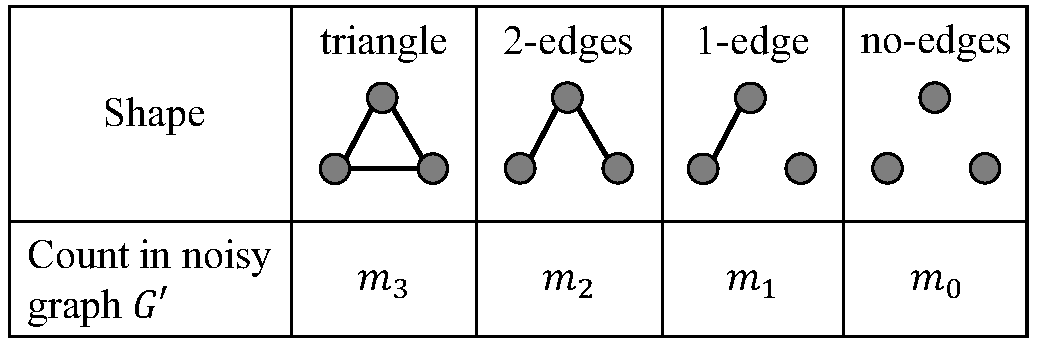
\includegraphics[width=0.9\linewidth]{fig/triplet_shape.pdf}
\caption{Four types of subgraphs with three nodes.}
\label{chap1-fig:triplet_shape}
\end{figure}

Through 
% some 
% a 
clever post-processing 
% method 
known as 
% an 
empirical estimation 
% method~
\cite{Kairouz_ICML16,Murakami_USENIX19,Wang_USENIX17},
we are able to obtain an unbiased estimate of $f_\triangle(G)$ 
% with access to just $P$. 
from $G'$. 
Specifically, a subgraph with three nodes can be divided into four types depending on the number of edges. 
Three nodes with three edges form a triangle. 
We refer to three nodes with two edges, one edge, and no edges as \textit{2-edges},  \textit{1-edge}, and  \textit{no-edges}, respectively. 
Figure~\ref{chap1-fig:triplet_shape} shows their shapes. 
% Let $m_3, m_2, m_1, m_0 \in \nnints$ be respectively the number of triangles, 2-edges, 1-edge, and no-edges in $G'$. 
% Note that $\sum_{i=0}^3 m_i = \binom{n}{3}$. 
% The expectation of 
$f_\triangle(G)$ can be expressed using $m_3$, $m_2$, $m_1$, and $m_0$ as follows:

\begin{proposition}\label{chap1-prop:triangle_emp}
  %Let $\mu = e^\epsilon$. 
  Let $G'=(V,E')$ be a noisy graph generated by applying the RR to the lower triangular part of $\bmA$.
  Let $m_3, m_2, m_1, m_0 \in \nnints$ be respectively the number of triangles, 2-edges, 1-edge, and no-edges in $G'$. 
  Then 
  \begin{align}
      %\textstyle{\mathbb{E}\left[ \frac{\mu^3}{(\mu-1)^3} m_3 - \frac{\mu^2}{(\mu-1)^3} m_2 + \frac{\mu}{(\mu-1)^3} m_1 - \frac{1}{(\mu-1)^3} m_0 \right] = f_\triangle(G).}
      \textstyle{\mathbb{E}\left[ \frac{e^{3\epsilon}}{(e^\epsilon-1)^3} m_3 \hspace{-0.5mm}-\hspace{-0.5mm} \frac{e^{2\epsilon}}{(e^\epsilon-1)^3} m_2 \hspace{-0.5mm}+\hspace{-0.5mm} \frac{e^\epsilon}{(e^\epsilon-1)^3} m_1 \hspace{-0.5mm}-\hspace{-0.5mm} \frac{1}{(e^\epsilon-1)^3} m_0 \right] \hspace{-0.5mm} = \hspace{-0.5mm} f_\triangle(G).}
      \label{chap1-eq:triangle_emp}
  \end{align}
\end{proposition}

% This significantly reduces the $l_2$ error. 
Therefore, the data collector can count $m_3$, $m_2$, $m_1$, and $m_0$ from $G'$, and calculate an unbiased estimate of $f_\triangle(G)$ by (\ref{chap1-eq:triangle_emp}). 
% Algorithm~\ref{chap1-alg:subgraph-rr} contains the precise way to do this.
In Appendix~\ref{chap1-sec:RR_emp}, we show that the $l_2$ loss is significantly reduced by this empirical estimation.

\setlength{\algomargin}{4mm}
\begin{algorithm}
  \SetAlgoLined
  \KwData{Graph $G$ 
  %described by distributed 
  represented as 
  neighbor lists $\bma_1,
    \ldots, \bma_n
  \in \{0,1\}^n$, privacy budget $\epsilon \in \nnreals$.}
  \KwResult{Private estimate of $f_\triangle(G)$.}
  \For{$i=1$ \KwTo $n$}{
    %$R_i \leftarrow (RR_{\epsilon}(a_i^1), \ldots, RR_{\epsilon}(a_i^{i-1}))$\;
    $R_i \leftarrow (RR_{\epsilon}(a_{i,1}), \ldots, RR_{\epsilon}(a_{i,i-1}))$\;
    $release(R_i)$\;
  }
  %$G' \leftarrow \texttt{UndirectedGraph}(R_1, \ldots, R_{i-1})$\;
  $G'=(V,E') \leftarrow \texttt{UndirectedGraph}(R_1, \ldots, R_n)$\;
  %\tcc{Counts $T_3,T_2,T_1,T_0$ in $P$.}
  \tcc{Counts $m_3,m_2,m_1,m_0$ in $G'$.}
  %$\hat{\textbf{m}} \leftarrow \texttt{CountSubgraphs}(G',3)$\;
  $(m_3, m_2, m_1, m_0) \leftarrow \texttt{Count}(G')$\;
  %$\mu \leftarrow e^\epsilon$\;
  %\KwRet{$\frac{1}{(\mu-1)^3}(\mu^3 m_3 -\mu^2 m_2 + \mu m_1 - m_0)$}
  \KwRet{$\frac{1}{(e^\epsilon-1)^3}(e^{3\epsilon} m_3 - e^{2\epsilon} m_2 + e^\epsilon m_1 - m_0)$}

  %\caption{CountSubgraphsRR\label{chap1-alg:subgraph-rr}}
  \caption{\alg{LocalRR$_\triangle$}\label{chap1-alg:subgraph-rr}}
\end{algorithm}

Algorithm~\ref{chap1-alg:subgraph-rr} shows this algorithm. 
In line 2, user $v_i$ applies the RR with privacy budget $\epsilon$ (denoted by $RR_\epsilon$) to $a_{i,1}, \ldots, a_{i,i-1}$ 
% (which corresponds to users $v_1, \ldots, v_{i-1}$ with smaller user IDs) 
in her neighbor list $\bma_i$, and outputs $R_i = (RR_\epsilon(a_{i,1}), \ldots, RR_\epsilon(a_{i,i-1}))$. 
In other words, we apply the RR to the lower triangular part of $\bmA$ and there is no overlap between edges sent by users. 
In line 5, the data collector uses a function (denoted by \texttt{UndirectedGraph}) 
that converts the bits of $(R_1, \ldots, R_n)$ into an undirected graph $G'
= (V, E')$ by adding edge $(v_i,v_j)$ with $i>j$ to $E'$ if and only if the $j$-th bit of
$R_i$ is $1$. 
Note that $G'$ is biased, as explained above. 
In line 6, the data collector uses a function (denoted by 
\texttt{Count}) that calculates $m_3$, $m_2$, $m_1$, and $m_0$ from $G'$. 
Finally, the data collector outputs the expression inside the expectation on
the left-hand side of (\ref{chap1-eq:triangle_emp}), which is an unbiased estimator for 
$f_\triangle(G)$ by Proposition~\ref{chap1-prop:triangle_emp}.
We denote this algorithm by \alg{LocalRR$_\triangle$}.

% One subtlety of Algorithm~\ref{chap1-alg:subgraph-rr} is that, since each edge is known by two users, releasing users' edges through the RR may result in disagreements over the noisy edges. User $i$ may claim that he is
% connected to $j$, and user $j$ may claim he is not connected to $i$. 
% To avoid this problem, we assume an ordering on users, and we let user $i$ ignore edge
% $(i,j)$ if $i<j$. This means each edge is the responsibility of just one user.
% Because edge $(i,j)$ is released by user $\max\{i,j\}$, it is technically a
% directed edge. Thus, we let $P$ be the undirected graph formed by taking the
% direction out of all noisy edges released (Line 5).


\smallskip
\noindent{\textbf{Theoretical properties.}}~~\alg{LocalRR$_\triangle$} 
% Algorithm~\ref{chap1-alg:subgraph-rr} 
provides the following guarantee.

\begin{theorem}\label{chap1-thm:subgraph-rr_LDP}
  \alg{LocalRR$_\triangle$} provides $\epsilon$-edge LDP and $\epsilon$-relationship DP.
\end{theorem}

\alg{LocalRR$_\triangle$} does not have the doubling issue (i.e., it provides not $2\epsilon$ but $\epsilon$-relationship DP), because we apply the RR to the lower triangular part of $\bmA$, as explained in Section~\ref{chap1-sub:LDP}.

Unlike the RR and empirical estimation for tabular data \cite{Kairouz_ICML16}, the expected $l_2$ loss of \alg{LocalRR$_\triangle$} is complicated. 
% due to the fact that multiple triangles can involve the same edge. 
To simplify the utility analysis, we assume that $G$ is generated from the Erd\"os-R\'enyi graph distribution $\bmG(n,\alpha)$ with edge existence probability $\alpha$; i.e., each edge in $G$ with $n$ nodes is independently generated with probability $\alpha \in [0,1]$.
% which generates $G=(V,E)$ with $|V|=n$ with

\begin{theorem}\label{chap1-thm:subgraph-rr}
  Let $\bmG(n,\alpha)$ be the Erd\"os-R\'enyi graph distribution with edge existence probability $\alpha \in [0,1]$. 
  Let $p = \frac{1}{e^\epsilon+1}$ and 
  $\beta = \alpha(1-p) + (1-\alpha)p$. 
  Let 
  %$A(G, \epsilon)$ 
  $\hf_{\triangle}(G, \epsilon)$ 
  be the output of 
  %Algorithm~\ref{chap1-alg:subgraph-rr}.
  \alg{LocalRR$_\triangle$}.
  %Suppose 
  %$G \sim \bmG(n,\frac{d_{max}}{n})$, 
  If 
  $G \sim \bmG(n,\alpha)$, 
  %the Erd\"os-R\'enyi graph
  %distribution with parameter $\frac{d_{max}}{n}$.  Then, 
  then for all 
  $\epsilon \in \nnreals$, 
  %$l_2^2(A(G,\epsilon),
  $\mathbb{E}[l_2^2(\hf_{\triangle}(G, \epsilon),
  f_\triangle(G))] = 
  %O(\frac{e^{6\epsilon}}{(e^\epsilon-1)^6}d_{max}n^3)$.
  O\left(\frac{e^{6\epsilon}}{(e^\epsilon-1)^6}\beta n^4\right)$.
  %Furthermore, Algorithm~\ref{chap1-alg:subgraph-rr} provides $\epsilon$-edge LDP.
\end{theorem}

% Note that Theorem~\ref{chap1-thm:subgraph-rr} is a statement about the expected 
% % average $l_2^2$ error
% $l_2$ loss 
% over graphs 
% % $G \sim \bmG(n,\frac{d_{max}}{n})$. 
% $G \sim \bmG(n,\alpha)$. 
% This is less ideal than the case of
% Theorem~\ref{chap1-thm:k-stars} which upper bounds the 
% % $l_2^2$ error 
% $l_2$ loss for all $G \in \calG$. 
% However, 
% % $\textbf{G}(n,\frac{d_{max}}{n})$ 
% $\textbf{G}(n,\alpha)$ 
% is considered a realistic model from which
% graphs of max degree $d_{max}$ are drawn, so Theorem~\ref{chap1-thm:subgraph-rr} is
% still 
% % a strong bound.
% valid. 

Note that we assume the Erd\"os-R\'enyi model only for the utility analysis of \alg{LocalRR$_\triangle$}, and do not assume this model for the other algorithms. 
The upper-bound of \alg{LocalRR$_\triangle$} in Theorem~\ref{chap1-thm:subgraph-rr} is less ideal than the upper-bounds of the other algorithms in that it does not consider all possible graphs $G \in \calG$. 
Nevertheless, we also show that the $l_2$ loss of \alg{LocalRR$_\triangle$} is roughly consistent with Theorem~\ref{chap1-thm:subgraph-rr} in our experiments using two real datasets (Section~\ref{chap1-sec:experiments}) and 
% artificial graphs based on 
the Barab\'{a}si-Albert graphs \cite{NetworkScience}, which have power-law degree distribution (Appendix~\ref{chap1-sec:BAGraph}). 

% The parameter $\alpha$ is very small in a sparse graph. 
% For example, it is reasonable to assume that $\alpha \leq \frac{d_{max}}{n} \ll 1$. 
% On the other hand, $\beta$ is a parameter in 
The parameters $\alpha$ and $\beta$ are edge existence probabilities in the original graph $G$ and noisy graph $G'$, respectively. 
Although $\alpha$ is very small in a sparse graph, $\beta$ can be large for small $\epsilon$. 
For example, if $\alpha \approx 0$ and $\epsilon=1$, then $\beta \approx \frac{1}{e+1} = 0.27$. 
% In this case, the expected $l_2$ loss of \alg{LocalRR$_\triangle$} can be expressed as: $O\left(\frac{e^{6\epsilon}}{(e^\epsilon-1)^6}d_{max} n^3\right)$.

Theorem~\ref{chap1-thm:subgraph-rr} states that for large $n$, the $l_2$ loss of \alg{LocalRR$_\triangle$} 
($=O(n^4)$) 
% ($=O(d_{max}n^3)$) 
is much larger than the $l_2$ loss of \alg{LocalRR$_k\star$} ($=O(n)$). 
This follows from the fact that user $v_i$ 
% cannot see any edge $(v_j, v_k) \in E$ in graph $G$ and 
is not aware of any triangle formed by $(v_i, v_j, v_k)$, as explained above. 

In contrast, counting $f_\triangle(G)$ in the centralized model is much easier because the data collector sees all triangles in $G$; i.e., the data collector knows $f_\triangle(G)$. 
% After we perform graph projection 
% \cite{Day_SIGMOD16,Kasiviswanathan_TCC13,Raskhodnikova_arXiv15} 
% so that each user's degree does not exceed $\td_{max}$, 
% the 
The 
% local 
% global 
sensitivity of $f_\triangle$ 
% becomes 
is 
at most $\td_{max}$ (after graph projection). 
% Therefore, as with $k$-stars, 
Thus, 
we can consider a simple algorithm that 
% performs graph projection so that each user's degree never exceeds $\td_{max}$, 
% and then 
% adds the Laplacian noise $\Lap(\td_{max}/\epsilon)$ 
% ($\td_{max} > d_{max}$) 
% to $f_{\triangle}(G)$, and 
outputs $f_{\triangle}(G) + \Lap(\td_{max}/\epsilon)$. 
We denote this algorithm by \alg{CentralLap$_{\triangle}$}. 
\alg{CentralLap$_{\triangle}$} attains the expected $l_2$ loss ($=$ variance) of $O\left(\frac{\td_{max}^2}{\epsilon^2}\right)$. 

% \colorB{In Section~\ref{chap1-sub:two_rounds}, we propose a two-rounds LDP algorithm for triangles to significantly reduce the $l_2$ loss in the local model.}

% In Algorithm~\ref{chap1-alg:subgraph-rr}, 
The large $l_2$ loss of \alg{LocalRR$_\triangle$} is caused by the fact that 
each edge is released independently with
some probability of being flipped. 
% Thus, 
In other words, 
there are three independent random
variables that influence 
% any subgraph of size $3$ in $P$. 
any triangle in $G'$. 
The next algorithm,
using interaction, 
% is able to reduce 
reduces 
this influencing number 
% to two, 
from three to one 
% because 
% a single 
by using the fact that 
a user 
% always 
knows 
% two edges of a subgraph of size 3.
the existence of two edges for any triangle that involves the user. 

% \ji{Can we combine the last and third-last paragraphs of this section?}
% \tm{It's a little bit difficult to me because 
% the explanation is in the order of ``Thm 4 --> one-round local (third-last) --> centralized (second-last) --> two-round local (last) (--> Sec 4.3)''. Instead, I shortened the third-last paragraph.}

% \subsection{Two-Rounds LDP Algorithms for Triangles}
\subsection{Two-Rounds Algorithms for Triangles}
% \colorB{Sequentially Interactive Graph LDP Algorithms}}
\label{chap1-sub:two_rounds}

\noindent{\textbf{Algorithm.}}~~Allowing for 
% sequential interaction, 
two-rounds interaction, 
we are able to compute $f_{\triangle}$ with
a significantly improved $l_2$ loss, albeit with a higher per-user
communication overhead.
As described in Section~\ref{chap1-sub:non-interactive_triangles}, it is impossible for user $v_i$ to see edge $(v_j, v_k) \in E$ in graph $G=(V,E)$ at the first round. 
However, if 
% each user $v_i$ applies the RR to her neighbor list $\bma_i$ as in \alg{LocalRR$_\triangle$} and 
the data collector publishes a noisy graph $G'=(V,E')$ calculated by \alg{LocalRR$_\triangle$} at the first round, then 
user $v_i$ can see a noisy edge $(v_j, v_k) \in E'$ in the noisy graph $G'$ at the second round. 
Then user $v_i$ can count the number of \textit{noisy triangles} formed by
$(v_i, v_j, v_k)$ such that $(v_i,v_j) \in E$, $(v_i,v_k) \in E$, and $(v_j,v_k)
\in E'$, and send the noisy triangle counts with the Laplacian noise to the data
collector in an analogous way to \alg{LocalLap$_{k\star}$}.
Since user $v_i$ always knows that two edges $(v_i,v_j)$ and $(v_i,v_k)$ exist in $G$, 
there is only one noisy edge in any noisy triangle 
(whereas all edges are noisy in \alg{LocalRR$_\triangle$}).
% edge $(v_j,v_k)$
% random variable 
% that influences the existence of the triangle $(v_i, v_j, v_k)$ in $G$. 
This is an intuition behind our proposed two-rounds algorithm. 

As with the RR in Section~\ref{chap1-sub:non-interactive_triangles}, simply counting the noisy triangles can introduce a bias. 
Therefore, we calculate an empirical estimate of $f_\triangle(G)$ from the noisy triangle counts. 
Specifically, 
% we calculate the expectation of 
the following is the empirical estimate of $f_\triangle(G)$: 
% can be expressed as follows:
% Specifically, assume that the data collector publishes a noisy graph $G'=(V,E')$ calculated by \alg{LocalRR$_\triangle$} with privacy budget $\epsilon_0 \in \nnreals$ at the first round. 
% Let $t_i \in \nnints$ be the number of triplets $(v_i, v_j, v_k)$ such that $j < i < k$, $(v_i,v_j) \in E$, $(v_i,v_k) \in E$, and $(v_j,v_k) \in E'$; i.e., 
% the number of noisy triangles user $v_i$ can see at the second round. 
% Here we count only triplets $(v_i, v_j, v_k)$ with $j < i < k$ to avoid counting the same triplet multiple times.
% Let $s_i \in \nnints$ be the number of triplets $(v_i, v_j, v_k)$ such that $j < i < k$, $(v_i,v_j) \in E$, and $(v_i,v_k) \in E$; i.e., 
% the number of $2$-stars of which user $v_i$ is a center. 
% Then the expectation of $f_\triangle(G)$ can be calculated from $\epsilon_0$, $t_i$, and $s_i$ as follows:

\begin{proposition}\label{chap1-prop:triangle_emp_2rounds}
  Let $G'=(V,E')$ be a noisy graph generated by applying the RR with privacy budget $\epsilon_1 \in \nnreals$   to the lower triangular part of $\bmA$.
  Let $p_1 = \frac{1}{e^{\epsilon_1}+1}$. 
  Let $t_i \in \nnints$ be the number of triplets $(v_i, v_j, v_k)$ such that 
  %$j < i < k$, 
  $j < k < i$, 
  $(v_i,v_j) \in E$, $(v_i,v_k) \in E$, and $(v_j,v_k) \in E'$.
  Let $s_i \in \nnints$ be the number of triplets $(v_i, v_j, v_k)$ such that 
  %$j < i < k$, 
  $j < k < i$, 
  $(v_i,v_j) \in E$, and $(v_i,v_k) \in E$. 
  Let $w_i = t_i - p_1 s _i$. 
  Then 
  \begin{align}
      %\textstyle{\mathbb{E}[f_\triangle(G)] = \frac{1}{1-2p_1} \sum_{i=1}^n (t_i - p_1 s_i)}.
      \textstyle{\mathbb{E}\left[ \frac{1}{1-2p_1} \sum_{i=1}^n w_i \right] = f_\triangle(G).}
      \label{chap1-eq:triangle_emp_2rounds}
  \end{align}
\end{proposition}

Note that in Proposition~\ref{chap1-prop:triangle_emp_2rounds}, 
we count only triplets $(v_i, v_j, v_k)$ with 
% $j < i < k$ 
$j < k < i$ 
% to avoid counting the same triplet multiple times. 
to use only the lower triangular part of $\bmA$. 
$t_i$ is the number of noisy triangles user $v_i$ can see at the second round. 
$s_i$ is the number of $2$-stars of which user $v_i$ is a center. 
Since $t_i$ and $s_i$ can reveal information about an edge in $G$, user $v_i$ adds the Laplacian noise to $w_i$ $(= t_i - p_1 s _i)$ in (\ref{chap1-eq:triangle_emp_2rounds}), and sends it to the data collector. 
Then the data collector calculates an unbiased estimate of $f_\triangle(G)$ by (\ref{chap1-eq:triangle_emp_2rounds}). 

% Instead of releasing each edge through 
% randomized
% response, user $i$ is given a specific query depending on $P_{i-1}$, the
% subgraph of $G$ on users $1$ through $i-1$ released through randomized response.
% Like Algorithm~\ref{chap1-alg:subgraph-rr}, we assume user $i$ ignores edge $(i,j)$ if
% $i<j$. The query to user $i$ is to noisily count the number of triangles of which he is
% a part, using two of his edges and one edge in $P_{i-1}$. He releases this
% number and a randomized response on his edges so that future users may build
% $P_{i}$. 

\setlength{\algomargin}{5mm}
\begin{algorithm}
  \SetAlgoLined
  \KwData{Graph $G$ 
  %described by distributed 
  represented as 
  neighbor lists $\bma_1,
    \ldots, \bma_n
    \in \{0,1\}^n$, two privacy budgets
  %$\epsilon_0,\epsilon_1 > 0$.}
  $\epsilon_1,\epsilon_2 > 0$, $\td_{max} \in \nnints$.}
  %\KwResult{Private count of number of triangles in $G$.}
  \KwResult{Private estimate of $f_\triangle(G)$.}
  %$\rho \leftarrow \frac{1}{e^{\epsilon_0}+1}$\;
  $p_1 \leftarrow \frac{1}{e^{\epsilon_1}+1}$\;
  \tcc{First round.}
  \For{$i=1$ \KwTo $n$}{
    %$ans_i \leftarrow 0$\;
    %$R_i \leftarrow (RR_{\epsilon_0}(a_i^1), \ldots, RR_{\epsilon_0}(a_i^{i-1}))$\;
    $R_i \leftarrow (RR_{\epsilon_1}(a_{i,1}), \ldots, RR_{\epsilon_1}(a_{i,i-1}))$\;
    $release(R_i)$\;
  }
  %$P_{i-1} \leftarrow \texttt{UndirectedGraph}(R_1, \ldots, R_{i-1})$\;
  $G'=(V,E') \leftarrow \texttt{UndirectedGraph}(R_1, \ldots, R_{i-1})$\;
  \tcc{Second round.}
  \For{$i=1$ \KwTo $n$}{
    $\bma_i \leftarrow \texttt{GraphProjection}(\bma_i, \td_{max})$\;
    %$t_i \leftarrow |\{(u,v) : u,v \in [i], u<v<i, a_{i}^u = a_{i}^v = 1,(u,v) \in P_{i-1}\}|$\;
    $t_i \leftarrow |\{(v_i,v_j,v_k) : 
    %j<i<k, a_{j,i} = a_{i,k} = 1, 
    j<k<i, a_{i,j} = a_{i,k} = 1, 
    (v_j,v_k) \in E'\}|$\;
    %$s_i \leftarrow |\{(u,v) : u,v \in [i], u<v<i, a_{i}^u = a_{i}^v = 1\}|$\;
    $s_i \leftarrow |\{(v_i,v_j,v_k) : 
    %j<i<k, a_{j,i} = a_{i,k} = 1\}|$\;
    j<k<i, a_{i,j} = a_{i,k} = 1\}|$\;
    %$w_i \leftarrow t_i - \rho s_i + Lap(\frac{d_{max}(1-\rho)}{\epsilon_1})$\;
    %$w_i \leftarrow t_i - p_1 s_i + \Lap(\frac{\td_{max}(1-p_1)}{\epsilon_2})$\;
    $w_i \leftarrow t_i - p_1 s_i$\;
    $\hw_i \leftarrow w_i + \Lap(\frac{\td_{max}}{\epsilon_2})$\;
    %$release(R_i, w_i)$\;
    $release(\hw_i)$\;
  }
  %$ans \leftarrow \frac{1}{1-2\rho}\sum_{i=1}^n w_i$\;
  \KwRet{$\frac{1}{1-2p_1}\sum_{i=1}^n \hw_i$}
  %\caption{CountSubgraphsTwoRound\label{chap1-alg:subgraph-interactive}}
  \caption{\alg{Local2Rounds$_\triangle$}}\label{chap1-alg:subgraph-interactive}
\end{algorithm}

Algorithm~\ref{chap1-alg:subgraph-interactive} contains the formal
description of this process. 
It takes as input a graph $G$, 
% (represented as neighbor lists $\bma_1, \ldots, \bma_n$), 
the privacy budgets $\epsilon_1, \epsilon_2 \in \nnreals$ at the first and second rounds, respectively, 
and 
% It also takes as input 
% an upper-bound $\td_{max}$ on the maximum degree $d_{max}$ of $G$ 
a non-negative integer $\td_{max} \in \nnints$. 
% in the same way as \alg{LocalLap$_{k\star}$}. 
% We will describe the private computation of $d_{max}$ with edge LDP at the end of Section~\ref{chap1-sub:two_rounds}. 
At the first round, we 
apply the RR to the lower triangular part of $\bmA$ 
(i.e., there is no overlap between edges sent by users) 
% . 
and use the \texttt{UndirectedGraph} function to 
obtain a noisy graph $G'=(V,E')$ by the RR in the same way as Algorithm~\ref{chap1-alg:subgraph-rr}. 
Note that $G'$ is biased. 
We calculate an unbiased estimate of $f_\triangle(G)$ from $G'$ at the second round.  
% Then we use the \texttt{UndirectedGraph} function, which makes an undirected graph $G'
% = (V, E')$ by adding edge $(i,j)$ with $i>j$ to $E'$ if and only if the $j$-th bit of $R_i$ is $1$. 

At the second round, each user $v_i$ 
calculates $\hw_i = w_i + \Lap(\frac{\td_{max}}{\epsilon_2})$ 
%  and 
by adding the Laplacian noise to $w_i$ 
% $(= t_i - p_1 s _i)$, 
in Proposition~\ref{chap1-prop:triangle_emp_2rounds} 
whose 
% local 
% global 
sensitivity is at most 
% $d_{max} (1-p_1)$, 
$\td_{max}$ 
% (after graph projection), 
(as we will prove in Theorem~\ref{chap1-thm:local2rounds_LDP}). 
Finally, we output $\frac{1}{1-2p_1}\sum_{i=1}^n \hw_i$, which is an unbiased estimate of $f_\triangle(G)$ by Proposition~\ref{chap1-prop:triangle_emp_2rounds}. 
We call this algorithm \alg{Local2Rounds$_\triangle$}.

% The intuitive reason Algorihtm~\ref{chap1-alg:subgraph-interactive} performs better than 
% Algorithm~\ref{chap1-alg:subgraph-rr} is that a noisy triangle is counted using two 
% noisy computations, the noisy edge in
% $P_{i-1}$ and user $i$'s noisy count. In Algorithm~\ref{chap1-alg:subgraph-rr}, each
% subgraph of size $3$ in $P$ is the result of three noisy computations.

\smallskip
\noindent{\textbf{Theoretical properties.}}~~\alg{Local2Rounds$_\triangle$} 
% Algorithm~\ref{chap1-alg:subgraph-interactive} 
has the following 
% performance 
guarantee.

\begin{theorem}\label{chap1-thm:local2rounds_LDP}
  %If the maximum degree $d_{max}$ of $G$ is at most $\td_{max}$, 
  \alg{Local2Rounds$_\triangle$}
  provides $(\epsilon_1 + \epsilon_2)$-edge LDP and $(\epsilon_1 + \epsilon_2)$-relationship DP.
\end{theorem}

As with \alg{LocalRR$_\triangle$}, \alg{Local2Rounds$_\triangle$} does not have the doubling issue; i.e., it provides $\epsilon$-relationship DP (not $2\epsilon$). 
This follows from the fact that we 
use only the lower triangular part of $\bmA$; 
% count each triplet $(v_i,v_j,v_k)$ only once; 
i.e., we assume 
%$j<i<k$ 
$j<k<i$ 
in counting $t_i$ and $s_i$. 

\begin{theorem}\label{chap1-thm:local2rounds}
  Let 
  %$A(G, d_{max}, \epsilon_0, \epsilon_1)$ 
  $\hf_{\triangle}(G, \epsilon_1, \epsilon_2, \td_{max})$ 
  be the output of 
  %Algorithm~\ref{chap1-alg:subgraph-interactive}. 
%   \alg{LocalRR$_\triangle$}. 
  \alg{Local2Rounds$_\triangle$}. 
  Then, for all 
  %$d_{max} \in \nats$,
  $\epsilon_1,\epsilon_2 \in \nnreals$, 
  $\td_{max} \in \nnints$,
  and $G\in \calG$ such that the
  maximum degree $d_{max}$ of $G$ is 
  at most 
  $\td_{max}$,
  %$l_2^2(A(G,d_{max},\epsilon_0,\epsilon_1) 
  $\mathbb{E}[l_2^2(\hf_{\triangle}(G, \epsilon_1, \epsilon_2, \td_{max}), f_\triangle(G))] 
  \leq
    O\left(\frac{e^{\epsilon_1}}{(1-e^{\epsilon_1})^2} \left(\td_{max}^3 n +
    \frac{e^{\epsilon_1}}{\epsilon_2^2}\td_{max}^2 n\right)\right)$.
\end{theorem}

Theorem~\ref{chap1-thm:local2rounds} means that for triangles, the $l_2$ loss 
% of \alg{LocalRR_$\triangle$} 
is reduced from $O(n^4)$ to $O(\td_{max}^3n)$ by introducing an additional round. 

% The upper and lower bounds on the $l_2$ losses for the central,
% % local non-interactive, 
% one-round local, 
% and 
% % local sequentially interactive 
% two-rounds local 
% models discussed in
% this section appear in Table~\ref{chap1-tab:perf}.

\smallskip
\noindent{\textbf{Private calculation of $d_{max}$.}}~~As with $k$-stars, we can privately calculate $d_{max}$ 
% with edge LDP 
by using the method described in Section~\ref{chap1-sub:non-interactive_k_stars}. 
Furthermore, the private calculation of $d_{max}$ does not increase the number of rounds; i.e., we can run \alg{Local2Rounds$_\triangle$} with the private calculation of $d_{max}$ in two rounds. 

Specifically, let $\epsilon_0 \in \nnreals$ be the privacy budget for the private calculation of $d_{max}$. 
At the first round, each user $v_i$ adds $\Lap(\frac{1}{\epsilon_0})$ to her degree $d_i$, 
% (i.e., number of ``$1$''s in her neighbor list $\bma_i$), 
and sends the noisy degree $\hd_i$ ($=d_i + \Lap(\frac{1}{\epsilon_0})$) to the data collector, along with the outputs $R_i = (RR_\epsilon(a_{i,1}), \ldots, RR_\epsilon(a_{i,i-1}))$ of the RR. 
The data collector calculates the noisy max degree $\hd_{max}$ ($= \max\{\hd_1,
\ldots, \hd_n\}$) as an estimate of $d_{max}$, and sends it back to all users. 
At the second round, we run \alg{Local2Rounds$_\triangle$} with input $G$ (represented as $\bma_1, \ldots, \bma_n$), $\epsilon_1$, $\epsilon_2$, and $\lfloor \hd_{max} \rfloor$. 

% At the second round, each user performs graph projection; i.e., if $d_i$ exceeds $\hd_{max}$, user $v_i$ randomly selects $\hd_{max}$ neighbors from her neighbor list $\bma_i$ (otherwise, user $v_i$ uses $\bma_i$ as it is). 
% Let $\bma'_i \in \{0,1\}^n$ be a neighbor list of user $v_i$ after this projection. 
% We run the second round part (lines $7$ to $12$) of \alg{Local2Rounds$_\triangle$} with input $\bma'_1, \ldots, \bma'_n$, $\epsilon_1$, $\epsilon_2$, 
% and $\hd_{max}$. 

At the first round, the calculation of $\hd_{max}$ provides $\epsilon_0$-edge LDP. 
% because each user's degree has the sensitivity $1$ under edge LDP. 
Note that it provides $2\epsilon_0$-relationship DP (i.e., it has the doubling issue) because one edge $(v_i,v_j) \in E$ affects both of the degrees $d_i$ and $d_j$ by 1. 
At the second round, \alg{LocalLap$_{k\star}$} provides $(\epsilon_1 + \epsilon_2)$-edge LDP and 
$(\epsilon_1 + \epsilon_2)$-relationship DP (Theorem~\ref{chap1-thm:local2rounds_LDP}). 
% because each user $v_i$'s degree in $\bma'_i$ never exceeds $\hd_{max}$. 
% (and then Theorem~\ref{chap1-thm:local2rounds_LDP} holds). 
Then by the composition theorem~\cite{DP}, this two-rounds algorithm provides $(\epsilon_0 + \epsilon_1 + \epsilon_2)$-edge LDP and $(2\epsilon_0 + \epsilon_1 + \epsilon_2)$-relationship DP. 
Although the total privacy budget is larger for relationship DP, the difference ($=\epsilon_0$) can be very small. 
In fact, we set $(\epsilon_0, \epsilon_1, \epsilon_2) = (0.1, 0.45, 0.45)$ or $(0.2, 0.9, 0.9)$ in our experiments (i.e., the difference is $0.1$ or $0.2$), and show that this algorithm provides almost the same utility as \alg{Local2Rounds$_\triangle$} with the true max degree $d_{max}$. 

\smallskip
\noindent{\textbf{Time complexity.}}~~We also note that \alg{Local2Rounds$_\triangle$} has an advantage over \alg{LocalRR$_\triangle$} in terms of the time complexity. 
% in addition to the expected $l_2$ loss. 

Specifically, \alg{LocalRR$_\triangle$} is inefficient because the data collector has to count the number of triangles $m_3$ in the noisy graph $G'$. 
Since the noisy graph $G'$ is dense (especially when $\epsilon$ is small) and there are $\binom{n}{3}$ subgraphs with three nodes in $G'$, the number of triangles is $m_3 = O(n^3)$. 
Then, the time complexity of \alg{LocalRR$_\triangle$} is 
% $O(n)$ for each user's part and $O(n^3)$ for the data collector's part, 
also $O(n^3)$, which is not practical for a graph with a large number of users $n$.
In fact, we implemented \alg{LocalRR$_\triangle$} ($\epsilon=1$) with C/C++ and measured its running time using one node of a supercomputer (ABCI: AI Bridging Cloud Infrastructure \cite{ABCI}). 
When $n=5000$, $10000$, $20000$, and $40000$, the running time was $138$, $1107$, $9345$, and $99561$ seconds, respectively; i.e., the running time was almost cubic in $n$. 
We can also estimate the running time for larger $n$. 
For example, when $n=1000000$, \alg{LocalRR$_\triangle$} ($\epsilon=1$) would require about $35$ years $(=1107 \times 100^3 /(3600 \times 24 \times 365))$. 
% Even if we use $1000$ nodes of the supercomputer (the ABCI has $1088$ nodes \cite{ABCI}) in parallel, \alg{LocalRR$_\triangle$} would require over $10$ days. 

In contrast, the time complexity of \alg{Local2Rounds$_\triangle$} 
% for each user 
is 
% $O(n)$ in the first round (l.3-4 in Algorithm~\ref{chap1-alg:subgraph-interactive}) and $O(d_{max}^2)$ in the second round (l.8-13 in Algorithm~\ref{chap1-alg:subgraph-interactive})). 
% $O(n + d_{max}^2)$ for each user's part and $O(n)$ for the data collector's part at the second round. 
$O(n^2 + n d_{max}^2)$\footnote{When we 
% want to 
evaluate 
% the utility of 
\alg{Local2Rounds$_\triangle$} in our experiments, 
% When we evaluate the utility of \alg{Local2Rounds$_\triangle$} on one computer, 
we can apply the RR to only edges that are required at the second round; i.e., $(v_j,v_k) \in G'$ in line 8 of Algorithm~\ref{chap1-alg:subgraph-interactive}. 
Then the time complexity of \alg{Local2Rounds$_\triangle$} 
% is 
can be reduced to 
$O(n d_{max}^2)$ in total. 
We also confirmed that when $n=1000000$, the running time of \alg{Local2Rounds$_\triangle$} was $311$ seconds on one node of the ABCI. 
% , which is $3.5 \times 10^6$ times faster than \alg{LocalRR$_\triangle$}. 
Note, however, that this does \textit{not} protect individual privacy, because it reveals the fact that users $v_j$ and $v_k$ are friends with $u_i$ to the data collector.}. 
% including the private calculation of $d_{max}$. 
The factor of $n^2$ comes from the fact that the size of the noisy graph $G'$ is $O(n^2)$. 
This also causes a large communication overhead, as explained below.
% Further reduction of the time complexity by compressing the graph size (e.g., via graph projection) is left for future work.}

\smallskip
\noindent{\textbf{Communication overhead.}}~~In 
% The \alg{Local2Rounds$_\triangle$} has a quadratic communication overhead.
\alg{Local2Rounds$_\triangle$}, each user need to see the noisy graph $G'$ 
of size $O(n^2)$ 
% with $O(n^2)$ bits 
to count $t_i$ and $s_i$. 
% must count $t_i$ and $s_i$ which depend on $G'$, the private graph computed in the first round. 
% Thus, each user must see $G'$, a graph with $O(n^2)$ bits. 
This results in a per-user communication overhead of $O(n^2)$. 
% We 
Although we 
do not simulate the communication overhead in our experiments that use \alg{Local2Rounds$_\triangle$}, 
% but 
the $O(n^2)$ overhead 
% would 
might 
limit its application in very large graphs. 
An interesting avenue of future work is how to compress the graph size (e.g., via graph projection or random projection) to reduce both the time complexity and the communication overhead.
% Again, compressing the graph size (e.g., via graph projection) is left for future work.

\begin{table*}
  \centering
\begin{tabular}{|l|l|p{3.5cm}|p{3cm}|l|l|l|}
  \hline
  & Centralized & \spantwo{One-round local} & Two-rounds local \\
  \hline
  & Upper Bound & Lower Bound & Upper Bound & Upper Bound \\ \hline

  $f_{k\star}$
  & $O\left( \frac{d_{max}^{2k-2}}{\epsilon^2} \right)$  
  &  $\Omega\left( \frac{e^{2\epsilon}}{(e^{2\epsilon}+1)^2}d_{max}^{2k-2}n \right)$ 
  &  $O\left( \frac{d_{max}^{2k-2}}{\epsilon^2}n \right)$ 
  &  $O\left( \frac{d_{max}^{2k-2}}{\epsilon^2}n \right)$ \\ \hline

 $f_\triangle$ 
  &  $O\left(\frac{d_{max}^2}{\epsilon^2}\right)$ 
  &  $\Omega\left( \frac{e^{2\epsilon}}{(e^{2\epsilon}+1)^2}d_{max}^2n \right)$
  &  $O\left(\frac{e^{6\epsilon}}{(e^{\epsilon}-1)^6}n^4\right)$ 
  (when $G \sim \bmG(n,\alpha)$)
  %(randomized bound)
  &  $O\left(\frac{e^\epsilon}{(e^\epsilon-1)^2}(d_{max}^3 n +
  \frac{e^\epsilon}{\epsilon^2}d_{max}^2 n)\right)$ \\ \hline

\end{tabular}
\caption{Bounds on $l_2$ losses for privately estimating $f_{k\star}$ and
$f_{\triangle}$ with $\epsilon$-edge LDP. For upper-bounds, we assume that  $\td_{max}=d_{max}$. 
For the centralized model, we use the Laplace mechanism. For
the one-round $f_\triangle$ algorithm, we apply Theorem~\ref{chap1-thm:subgraph-rr} 
with constant $\alpha$. For the two-round protocol $f_\triangle$ algorithm, we
apply Theorem~\ref{chap1-thm:local2rounds} with
$\epsilon_1=\epsilon_2=\frac{\epsilon}{2}$. }\label{chap1-tab:perf}
\end{table*}

\subsection{Lower Bounds}
\label{chap1-sub:lower_bounds}

We show a general lower bound on the $l_2$ loss of private estimators $\hat{f}$ of
real-valued functions $f$ in the one-round LDP model. Treating $\epsilon$ as a
constant, we have shown that 
when $\td_{max}=d_{max}$, 
% for graphs $G$ of maximum degree $d_{max}$,
the expected $l_2$ loss of \alg{LocalLaplace$_{k\star}$} is 
% $l_2^2(\alg{LocalLaplace$_{k\star}$}(G), f_{k\star}(G)) = 
$O(nd_{max}^{2k-2})$
(Theorem~\ref{chap1-thm:k-stars}). 
% and 
% the expected $l_2$ loss of 
% \alg{Local2Rounds$_\triangle$} is 
% \alg{LocalRR$_\triangle$} is 
%$l_2^2(\alg{LocalRR$_\triangle$}(G),
% f_{k\star}(G) ) = 
% $O(nd_{max}^2)$ 
% $O(nd_{max}^3)$ 
% $O(n^4)$ 
% (Theorem~\ref{chap1-thm:local2rounds}). 
% (Theorem~\ref{chap1-thm:subgraph-rr}). 
However, in
the centralized 
% edge-DP 
model, we can use
the Laplace mechanism with sensitivity 
$2\binom{d_{max}}{k-1}$ 
% and 
%$d_{max}^2$,
% $d_{max}$ 
% respectively, 
to obtain $l_2^2$ errors of $O(d_{max}^{2k-2})$ 
% and
% $O(d_{max}^2)$, respectively 
for $f_{k\star}$. 
% and $f_\triangle$. 
Thus, we ask
if 
% the factors of $n$ are 
the factor of $n$ is 
necessary 
% in the local model. 
in the one-round LDP model.

We 
% partially 
answer this question affirmatively.
We show for many types of queries $f$, there is a lower bound on 
% $l_2^2(f(\bmA), \hf(\bmA))$ 
$l_2^2(f(G), \hf(G))$ 
for any private estimator $\hf$ of the form
\begin{equation}\label{chap1-eq:one-round-lower}
%   \hf(\bmA) = \tilde{f}(\calR_1(\bma_1), \ldots, \calR_n(\bma_n)).
  \hf(G) = \tilde{f}(\calR_1(\bma_1), \ldots, \calR_n(\bma_n)),
\end{equation}
where 
$\calR_1, \ldots, \calR_n$ satisfy 
% $\epsilon$-relationship or $\epsilon$-edge DP 
$\epsilon$-edge LDP or $\epsilon$-relationship DP 
and $\tilde{f}$ is an aggregate function that takes $\calR_1(\bma_1), \ldots, \calR_n(\bma_n)$ as input and outputs $\hf(G)$. 
Here we assume that $\calR_1, \ldots, \calR_n$ 
% and 
are independently run, meaning that they are in the one-round
setting.
% 
% Our lower bound has the form of $\Omega(nD^2)$, where $D$ is a positive real
% number depending on $f$ that is similar to, but stronger than, the global sensitivity $GS_f$.
% Global sensitivity by itself cannot provide a strong lower bound in the
% local model. As a counterexample, if $f$ were the function that is always $0$ or $GS_f$,
% then an estimator $\hf$ that predicts $0$ would satisfy
% $l_2^2(f(\bmA),\hf(\bmA)) = O(GS_f^2)$
% for all adjacency matrices $\bmA$. 
% 
% Instead, we 
For our 
%this 
lower bound,
% we consider $f$ to be a function on graphs. 
% not matrices. 
% Then 
% We 
we 
require 
that 
input edges to $f$ 
% to 
be ``independent'' in the sense that 
% and 
adding an edge to an input graph $G$  
independently 
% increase 
change 
$f$ by at least $D \in \reals$. 
% over a set of input graphs. 
% Notice that we consider $f$ to be a function on graphs, not
% matrices, for this lower bound. 
The specific structure of input graphs we require is as follows:

\begin{definition}\label{chap1-def:mono-cube}[$(n,D)$-independent cube for $f$]
  Let 
  %$D \in \reals$. 
  $D \in \nnreals$. 
  For 
  %$k \in \nats$, 
  $\kappa \in \nats$, 
  let $G=(V,E) \in \calG$ be a graph on 
  %$n = 2k$ 
  $n = 2\kappa$ 
  nodes, and let 
  %$M = \{(v_{i_1}, v_{i_2}),(v_{i_3},v_{i_4}),\ldots,(v_{i_{2k-1}},v_{i_{2k}})\}$ 
  $M = \{(v_{i_1}, v_{i_2}),(v_{i_3},v_{i_4}),\ldots,(v_{i_{2k-1}},v_{i_{2\kappa}})\}$ 
  for integers $i_j \in [n]$ 
  %denote 
  be 
  a set of edges such that each of $i_1, \ldots, i_{2\kappa}$ is distinct (i.e., perfect matching on the nodes).
%   a perfect
%   matching on the 
%   nodes, 
%   meaning each 
%   of $i_1, \ldots, i_{2k}$ 
%   is distinct. 
  %Furthermore,
  Suppose that 
  %the perfect matching 
  $M$ is disjoint from 
  $E$; 
  %$G$; 
  i.e., 
  % , meaning 
  %$(v_{i_{2j-1}}, v_{i_{2j-2}}) \notin G$. 
  %$(v_{i_{2j-1}}, v_{i_{2j}}) \notin G$ 
  $(v_{i_{2j-1}}, v_{i_{2j}}) \notin E$ 
  for any 
  %$j\in[k]$. 
  $j\in[\kappa]$. 
  Let 
%   $\calA = \{G \cup N : N \subseteq M\}$.
  $\calA = \{(V, E \cup N): N \subseteq M\}$.
  %Notice 
  Note that 
  $\calA$ is a set of 
  %$2^k$ 
  $2^\kappa$ 
  graphs.
  We say $\calA$ 
  %defines 
  %forms 
  is 
  an \emph{$(n,D)$-independent cube for $f$} if for all
  %$G_1, G_2 \in \calA$ such that $|G_1| + 1 = |G_2|$, 
  $G'=(V,E') \in \calA$, 
  %$G \in \calA$, 
  we have
  \[
    % f(G) = f(G') + \sum_{e \in M} \textbf{1}[e \in G] C_e
    f(G') = f(G) + \sum_{e \in E' \cap M} C_e,
  \]
  where $C_e \in \reals$ satisfies $|C_e| \geq D$ for any $e \in M$.
%   for non-negative real numbers 
%   $\{C_e : e \in M, |C_e| \geq D\}$.}
%   for real numbers 
%   $\{C_e : e \in M\}$ satisfying $|C_e| \geq D$.
\end{definition}

\begin{figure}[t]
  \centering
%   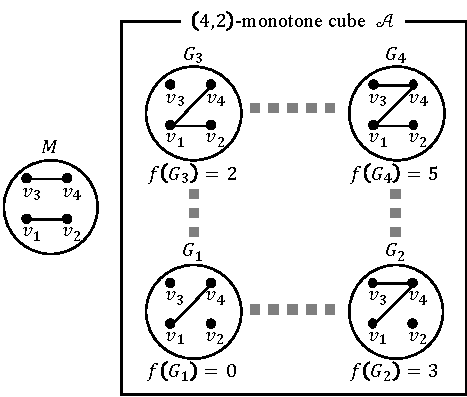
\includegraphics[width=0.88\linewidth]{fig/MonoCube.pdf}
  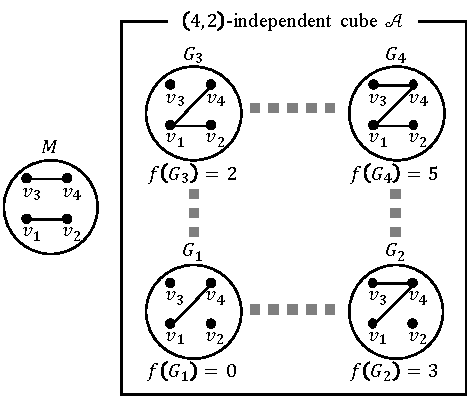
\includegraphics[width=0.9\linewidth]{fig/IndCube.pdf}
  \caption{
    $(4,2)$-independent cube $\calA$ for $f$. 
    In this example, $M = \{(v_1,v_2),(v_3,v_4)\}$, $G_1=(V,E)$, $\calA = \{(V, E \cup N): N \subseteq M\}$, 
    $C_{(v_1,v_2)}=2$, and $C_{(v_3,v_4)}=3$.
    %Definition~\ref{chap1-def:mono-cube} requires that $f$ increase by at least $D=2$ along the dotted gray lines, which it does.
    Adding $(v_1,v_2)$ and $(v_3,v_4)$ increase $f$ by $2$ and $3$, respectively.
  }\label{chap1-fig:mono-cube}
\end{figure}

\begin{figure}[t]
  \centering
  %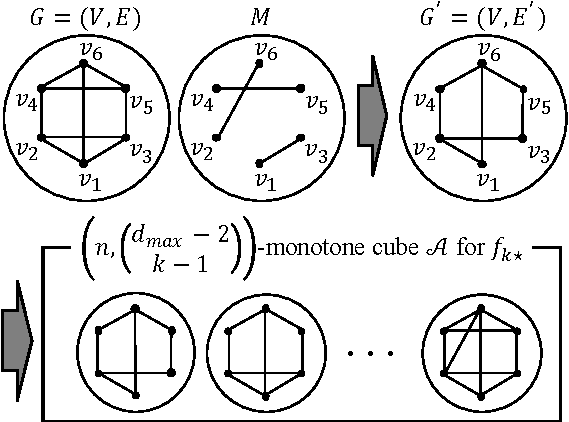
\includegraphics[width=0.88\linewidth]{fig/MonoCube_kstar.pdf}
  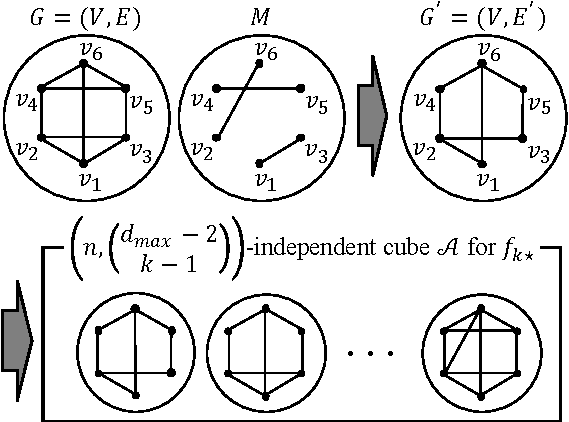
\includegraphics[width=0.9\linewidth]{fig/IndCube_kstar.pdf}
  \caption{
    Construction of an independent cube for a $k$-star function ($n=6$, $d_{max}=4$). 
    From a 
    %$(d_{max} - 1)$-
    $3$-regular graph $G=(V,E)$ and $M=\{(v_1,v_3),(v_2,v_6),(v_4,v_5)\}$, we make a graph $G'=(V,E')$ such that $E' = E \setminus M$. 
    Then $\calA = \{(V, E' \cup N): N \subseteq M\}$ forms an
    $(n, 2\binom{d_{max}-2}{k-1})$-independent cube for $f_{k\star}$.
  }\label{chap1-fig:mono-cube_kstar}
\end{figure}

% We show how to construct an $(n, \binom{d_{max}-3}{k-1})$ monotone cube
% $\mathcal{A}_{k\star}$ for
% $f_{k\star}$. First, we have to take care of a technicality.
% Note that $f_{k\star}(\bmA)$ only operates on symmetric graphs. We extend it to 
% general graphs in a natural way: let $f_{k\star}^{ext}(\bmA)$
% count the number of pointed-out $k$-stars in $\bmA$. Let
% $sym(\mathcal{A})$ be only those matrices in $\mathcal{A}$ that are symmetric,
% corresponding to undirected graphs. We show in the Appendix
% that if $\hf$ privately estimates $f_{k\star}^{ext}$ in the one-round
% edge LDP model, then there is a private estimator $\hat{g}$ that estimates
% $f_{k\star}$ in the one-round edge-LDP model such that
% \begin{multline}\label{chap1-eq:sym-lower-bound}
%   \E_{\bmA \sim U(\mathcal{A}_{k\star})}[l_2^2(f^{ext}_{k\star}(\bmA),
%   \hf(\bmA))] \\ \leq 
%   \E_{\bmA \sim U(sym(\mathcal{A}_{k\star}))} [l_2^2(f_{k\star}(\bmA),
%   \hf(\bmA))] + O(D^2)
% \end{multline}

Such a set of inputs has an ``independence'' property because,
regardless of which edges from $M$ has been added before, adding edge $e \in M$
always changes $f$ by $C_e$. 
Figure~\ref{chap1-fig:mono-cube} shows an example of a $(4,2)$-independent cube for $f$. 

% For example, 
We can also construct 
% an
% Our 
% $(n,\binom{d_{max}-3}{k-1})$ 
% $(n,\binom{d_{max}-4}{k-1})$ 
a independent cube for 
a $k$-star function 
% on directed graphs 
as follows. 
% $f_{k\star}^{ext}$ is the
% following:
% Assume $d_{max}$ and $n$ are both even. 
Assume that $n$ is even. 
It is well known in graph theory that if $n$ is even, then 
for any $d\in[n-1]$, there exists a 
$d$-regular graph where every node has degree $d$ \cite{Ganesan_arXiv18}. 
%Assume $n$ and $d_{max}$ are even and 
Therefore, there exists a 
% Let $G \in \calG$ be a $(d_{max}-1)$-regular graph 
$(d_{max}-1)$-regular graph $G=(V,E)$ 
of size $n$. 
% or a graph 
% in which every node has degree $d_{max}-1$. 
% It is a standard result in graph theory that 
% for any $d\in[n-1]$, 
% $d$-regular graphs exist 
% % for all $d$ 
% when $n$ is even.
Pick an arbitrary perfect matching $M$ on the nodes. Now, let 
% $G' = G \setminus M$. 
$G' = (V,E')$ such that $E' = E \setminus M$. 
Every node in $G'$ has degree between $d_{max}-2$ and $d_{max}-1$. 
Adding an edge in $M$ to $G'$ will produce at least
$2\binom{d_{max}-2}{k-1}$ new $k$-stars.
%the resulting graph be $\bmA = \{\bma_1,\ldots, \bma_n\}$.
%The collection $\prod_{i=1}^n \{\bma_i, \bma_i'\}$ (where the product is the Cartesian product) 
%forms an
% $(n,\binom{d_{max}-3}{k-1})$ 
% $(n,\binom{d_{max}-4}{k-1})$ 
Thus, $\calA = \{(V, E' \cup N): 
% G' \cup N : 
N \subseteq M\}$ forms an
$(n, 2\binom{d_{max}-2}{k-1})$-independent cube for $f_{k\star}$. 
% for $f_\triangle^{ext}$ 
% $\binom{d_{max}-3}{k-1}$ 
% $\binom{d_{max}-4}{k-1}$ 
%Similarly, for even natural number $l \in \nats$ such that $d_{max}>l+2$, we can construct an $(n,\binom{d_{max}-l-2}{k-1})$ monotone cube from the adjacency matrix of a collection of cliques of size $d_{max}-l$.
Note that the maximum degree of each graph in $\calA$ is at most $d_{max}$. 
Figure~\ref{chap1-fig:mono-cube_kstar} shows how to construct an independent cube for a $k$-star function when $n=6$ and $d_{max}=4$. 

% Let $U(\mathcal{A})$ be the uniform distribution over an $(n,D)$ monotone cube $\mathcal{A}$. 
Using the structure that the $(n,D)$-independent cube imposes on $f$,
we can prove a lower bound:
\begin{theorem}\label{chap1-thm:lower-bound}
  Let 
  %$\hf(\bmA)$ 
  $\hf(G)$ 
  have the form of~\eqref{chap1-eq:one-round-lower}, 
  where $\calR_1, \ldots, \calR_n$ are independently run.
  %Assume that 
  %$(\calR_1, \ldots, \calR_n)$ 
  %satisfy 
  %provide 
  %$\epsilon$-relationship DP. 
  %and are independently run.
  Let $\cal{A}$ be an $(n,D)$-independent cube for $f$. 
  If 
  $(\calR_1, \ldots, \calR_n)$ 
  provides 
  $\epsilon$-relationship DP, 
  then 
  %, with 
  %$\bmA$ 
  %$G$ 
  %uniformly drawn from $\calA$, 
  we have
  \[
    % \E_{\bmA, \calR_1, \ldots, \calR_n}[l_2^2(f(\bmA), \hf(\bmA))] =
    % \Omega(\frac{e^{\epsilon}}{(e^{\epsilon}+1)^2}nD^2).
    \frac{1}{\calA} \sum_{G \in \calA} \E[l_2^2(f(G), \hf(G))] =
    \Omega\left(\frac{e^{\epsilon}}{(e^{\epsilon}+1)^2}nD^2\right).
  \]
\end{theorem}

% \begin{corollary}\label{chap1-cor:lower-bound2}
%   If $\hf$ satisfies $\epsilon$-edge LDP in the one-round model, then $\E_{\bmA \sim U(\mathcal{A})}[l_2^2(f(\bmA), \hf(\bmA))] =
%   \Omega(\min\{1, \frac{e^{4\epsilon}}{(e^{4\epsilon}-1)^2}\}nD^2)$.
% \end{corollary}

A corollary of Theorem~\ref{chap1-thm:lower-bound} is that if $\calR_1, \ldots,
\calR_n$ satisfy $\epsilon$-edge LDP, then they satisfy $2\epsilon$
-relationship DP and thus for edge LDP we have a lower bound of
$\Omega\left(\frac{e^{2\epsilon}}{(e^{2\epsilon}+1)^2}nD^2\right)$.
% predictor $\hf$ predicting the average $\E_{\bmA \sim U(\mathcal{A})}[f(\bmA)]$
% will satisfy $\E_{\bmA \sim U(\mathcal{A})}[l_2^2(f(\bmA), \hf(\bmA))] =
% O(nD^2)$ regardless of $\epsilon$. To overcome this problem, one would have to 
% consider a different input structure for $f$ than the $(n,D)$ monotone cube, 
% but we leave this for future work.

Theorem~\ref{chap1-thm:lower-bound}, combined with the fact that there exists an
% $(n,\binom{d_{max}-2}{k-1})$ 
$(n,2\binom{d_{max}-2}{k-1})$-independent cube for 
a $k$-star function 
% $f_{k\star}$ 
% and~\eqref{chap1-eq:sym-lower-bound}, 
implies Corollary~\ref{chap1-cor:kstars-lb}. 
% (see Appendix~\ref{chap1-sub:proof_cor_kstars-lb} for details).
In Appendix~\ref{chap1-sub:cube_triangle}, we also construct an $(n, \frac{d_{max}}{2}-2)$
independent cube 
for $f_\triangle$ and establish a lower bound of 
$\Omega(\frac{e^{2\epsilon}}{(e^{2\epsilon}+1)^2} nd_{max}^2)$ for
$f_\triangle$. 

The upper and lower bounds on the $l_2$ losses 
% for the central,
% local non-interactive, 
% one-round local, 
% and 
% local sequentially interactive 
% two-rounds local 
% models discussed 
shown in
this section appear in Table~\ref{chap1-tab:perf}.
